% Versão 24/06/2020

% Este documento destina-se a servir como modelo para a produção de documentos
% de pesquisa do PPGINF/UFPR, como projetos, dissertações e teses. A classe de
% documento se chama "ppginf" (arquivo ppginf.cls) e define o formato básico do
% documento. O texto está organizado em capítulos que são colocados em
% subdiretórios separados. São definidos exemplos para a inclusão de figuras,
% códigos-fonte e a definição de tabelas.
%
% Produzido por Carlos Maziero (maziero@inf.ufpr.br).

%=====================================================

% Opções da classe ppginf:
%
% - defesa    : versão para entregar à banca; tem espaçamento 1,5
%               e omite algumas páginas iniciais (agradecimentos, etc)
% - final     : versão pós-defesa, para enviar à biblioteca;
%               tem espaçamento simples e todas as páginas iniciais.
% - oneside   : somente frente; use quando for gerar somente o PDF.
% - twoside   : frente/verso; use se precisar de uma versão impressa.
% - metadados : inclui metadados no PDF (por default não inclui)
% - ...       : demais opções aceitas pela classe "book"

% ATENÇÂO: este modelo tem suporte para português e inglês.
% As duas línguas devem ser informadas como opção da classe;
% a língua principal do documento deve vir POR ÚLTIMO.

% Versão de defesa em português
%\documentclass[defesa,oneside,english,brazilian]{ppginf}

% Versão de defesa em inglês
\documentclass[defesa,oneside,brazilian,english]{ppginf}
% Versão final em inglês
%\documentclass[final,oneside,brazilian,english]{ppginf}


% Versão final em PDF para a biblioteca da UFPR (português e inglês)
%\documentclass[final,oneside,english,brazilian]{ppginf}
%\documentclass[final,oneside,brazilian,english]{ppginf}

% Versão final para impressão (frente/verso)
%\documentclass[final,twoside,english,brazilian]{ppginf}

% configurações de diversos pacotes, inclusive a fonte usada no texto
% Pacotes usados neste documento e suas respectivas configurações

% ------------------------------------------------------------------------------

% Definição de fontes

% formato dos arquivos-fonte (utf8 no Linux e latin1 no Windows)
\usepackage[utf8]{inputenc}	% arquivos LaTeX em Unicode (UTF8)

% usar codificação T1 para ter caracteres acentuados corretos no PDF

% fonte usada no corpo do texto (pode alterar, mas descomente apenas uma)
%\usepackage{newtxtext,newtxmath}	% Times (se não tiver, use mathptmx)
%\usepackage{lmodern}			% Computer Modern (fonte clássico LaTeX)
\usepackage{kpfonts}			% Kepler/Palatino (idem, use mathpazo)
%\renewcommand{\familydefault}{\sfdefault} % Arial/Helvética (leia abaixo)

% A biblioteca central da UFPR recomenda usar Arial, seguindo a recomendação da
% ABNT. Essa é uma escolha ruim, pois fontes sans-serif são geralmente inade-
% quados para textos longos e impressos, sendo melhores para páginas Web.
% http://www.webdesignerdepot.com/2013/03/serif-vs-sans-the-final-battle/.

% fontes usadas em ambientes específicos
\usepackage[scaled=0.9]{helvet}		% Sans Serif
\usepackage{courier}			% Verbatim, Listings, etc

% ------------------------------------------------------------------------------

% inclusão de figuras em PDF, PNG, PS, EPS
\usepackage{graphicx}

% subfiguras (subfigure is deprecated, don't use it)
\usepackage[labelformat=simple]{subcaption}
\renewcommand\thesubfigure{(\alph{subfigure})}

% ------------------------------------------------------------------------------

% inclusão/formatação de código-fonte (programas)
\usepackage{listings}
\lstset{language=c}
\lstset{basicstyle=\ttfamily\footnotesize,commentstyle=\textit,stringstyle=\ttfamily}
\lstset{showspaces=false,showtabs=false,showstringspaces=false}
\lstset{numbers=left,stepnumber=1,numberstyle=\tiny}
\lstset{columns=flexible,mathescape=true}
\lstset{frame=single}
\lstset{inputencoding=utf8,extendedchars=true}
\lstset{literate={á}{{\'a}}1  {ã}{{\~a}}1 {à}{{\`a}}1 {â}{{\^a}}1
                 {Á}{{\'A}}1  {Ã}{{\~A}}1 {À}{{\`A}}1 {Â}{{\^A}}1
                 {é}{{\'e}}1  {ê}{{\^e}}1 {É}{{\'E}}1  {Ê}{{\^E}}1
                 {í}{{\'\i}}1 {Í}{{\'I}}1
                 {ó}{{\'o}}1  {õ}{{\~o}}1 {ô}{{\^o}}1
                 {Ó}{{\'O}}1  {Õ}{{\~O}}1 {Ô}{{\^O}}1
                 {ú}{{\'u}}1  {Ú}{{\'U}}1
                 {ç}{{\c{c}}}1 {Ç}{{\c{C}}}1 }

% ------------------------------------------------------------------------------

% formatação de algoritmos
\usepackage{algorithm,algorithmic}
\IfLanguageName{brazilian} {\floatname{algorithm}{Algoritmo}}{}
\renewcommand{\algorithmiccomment}[1]{~~~// #1}
%\algsetup{linenosize=\footnotesize,linenodelimiter=.}

% ------------------------------------------------------------------------------

% formatação de bibliografia
\usepackage{natbib}			% bibliografia no estilo NatBib
% \IfLanguageName{brazilian}
% {\bibliographystyle{apalike-ptbr}}	% formato em português
% {\bibliographystyle{apalike}}		% formato em inglês

% Estilos de bibliografia recomendados (só descomentar um estilo!)
% Mais infos: https://pt.sharelatex.com/learn/Bibtex_bibliography_styles
%
%\bibliographystyle{apalike-ptbr}	% [Maziero et al., 2006]
%\bibliographystyle{alpha}		% [Maz06]
%\bibliographystyle{plainnat}		% vide Google "LaTeX Natbib"
%\bibliographystyle{plain}		% [1] ordem alfabética
\bibliographystyle{unsrt}		% [1] ordem de uso no texto

% no estilo "unsrt", evita que citações nos índices sejam consideradas
%\usepackage{notoccite}

\renewcommand{\cite}{\citep}	% \cite deve funcionar como \citep
%\bibpunct{[}{]}{;}{a}{}{,}	% caracteres usados nas referências

% ------------------------------------------------------------------------------

% fontes adicionais
\usepackage{amsmath}		% pacotes matemáticos
\usepackage{amsfonts}		% fontes matemáticas 
%\usepackage{amssymb}		% símbolos 

% ------------------------------------------------------------------------------

% pacotes diversos
\usepackage{alltt,moreverb}	% mais comandos no modo verbatim
\usepackage{lipsum}		% gera texto aleatório (para os exemplos)
\usepackage{currfile}		% infos sobre o arquivo/diretório atual
\usepackage[final]{pdfpages}	% inclusão de páginas em PDF
\usepackage{longtable}		% tabelas multi-páginas (tab símbolos/acrônimos)

% ------------------------------------------------------------------------------



%=====================================================

\begin {document}

% Principais dados, usados para gerar as páginas iniciais.
% Campos não utilizados podem ser removidos ou comentados.

% título
\title{Using 3D gaze estimation models to monitor drivers' attention}

% palavras-chave e keywords (p/ resumo, abstract e metadados do PDF)
%\pchave{Palavra-chave 1. Palavra-chave 2. Palavra-chave 3.}
% \keyword{Gaze Estimation. Computer Vision. Image Processing.}
\keyword{Gaze estimation. Driver attention. Computer vision.}


% autoria
\author{Gabriel Nascarella Hishida do Nascimento}
\advisor{Prof. Eduardo Todt}

% instituição
\IfLanguageName{brazilian}
  { \instit{UFPR}{Universidade Federal do Paraná} }
% a Bib/UFPR exige que tudo seja em português, exceto o título :-(
%  { \instit{UFPR}{Federal University of Paraná} }
  { \instit{UFPR}{Universidade Federal do Paraná} }

% área de concentração (default do PPGInf, não mudar)
\IfLanguageName{brazilian}
  { \field{Ciência da Computação} }
% a Bib/UFPR exige que tudo seja em português, exceto o título :-(
%  { \field{Computer Science} }
  { \field{Ciência da Computação} }

% data (só o ano)
\date{2022}

% local
\IfLanguageName{brazilian}
  { \local{Curitiba PR} }
% a Bib/UFPR exige que tudo seja em português, exceto o título :-(
%  { \local{Curitiba PR - Brazil} }
  { \local{Curitiba PR} }

% imagem de fundo da capa (se não desejar, basta comentar)
\coverimage{0-iniciais/fundo-capa.jpg}

%=====================================================

%% Descrição do documento (obviamente, descomentar somente UMA!)

% Por exigência da biblioteca da UFPR, a descrição do documento deve ser
% em português, mesmo em documentos em outras línguas. Vá entender...

% tese de doutorado
%\descr{Tese apresentada como requisito parcial à obtenção do grau de Doutor em Ciência da Computação no Programa de Pós-Graduação em Informática, Setor de Ciências Exatas, da Universidade Federal do Paraná}

% exame de qualificação de doutorado
%\descr{Documento apresentado como requisito parcial ao exame de qualificação de Doutorado no Programa de Pós-Graduação em Informática, Setor de Ciências Exatas, da Universidade Federal do Paraná}

% dissertação de mestrado
%\descr{Dissertação apresentada como requisito parcial à obtenção do grau de Mestre em Informática no Programa de Pós-Graduação em Informática, Setor de Ciências Exatas, da Universidade Federal do Paraná}

% exame de qualificação de mestrado
%\descr{Documento apresentado como requisito parcial ao exame de qualificação de Mestrado no Programa de Pós-Graduação em Informática, Setor de Ciências Exatas, da Universidade Federal do Paraná}

% trabalho de conclusão de curso
\descr{Trabalho apresentado como requisito parcial à conclusão do Curso de Bacharelado em Ciência da Computação, Setor de Ciências Exatas, da Universidade Federal do Paraná}

% trabalho de disciplina
%\descr{Trabalho apresentado como requisito parcial à conclusão da disciplina XYZ no Curso de Bacharelado em XYZ, Setor de Ciências Exatas, da Universidade Federal do Paraná}

% doctorate thesis
%\descr{Thesis presented as a partial requirement for the degree of Doctor in Computer Science in the Graduate Program in Informatics, Exact Sciences Sector, of the Federal University of Paraná, Brazil}

% doctorate qualification
%\descr{Document presented as a partial requirement for the doctoral qualification exam in the Graduate Program in Informatics, Exact Sciences Sector, of the Federal University of Paraná, Brazil}

% MSc dissertation
%\descr{Dissertation presented as a partial requirement for the degree of Master of Sciences in Informatics in the Graduate Program in Informatics, Exact Sciences Sector, of the Federal University of Paraná, Brazil.}

% MSc qualification
%\descr{Document presented as a partial requirement for the Master of Sciences qualification exam in the Graduate Program in Informatics, Exact Sciences Sector, of the Federal University of Paraná, Brazil}

%=====================================================

% define estilo das páginas iniciais (capas, resumo, sumário, etc)
\frontmatter
\pagestyle{frontmatter}

% produz capa e folha de rosto
\titlepage

% páginas que só aparecem na versão final (a inclusão é automática)
% IMPORTANTE: o conteúdo exato da ficha catalográfica é preparada pela
% Biblioteca da UFPR. Não "invente" um conteúdo para ela!

\begin{ficha}	% só gera conteúdo se for na versão final

% inclusão da ficha catalográfica final (arquivo PDF)
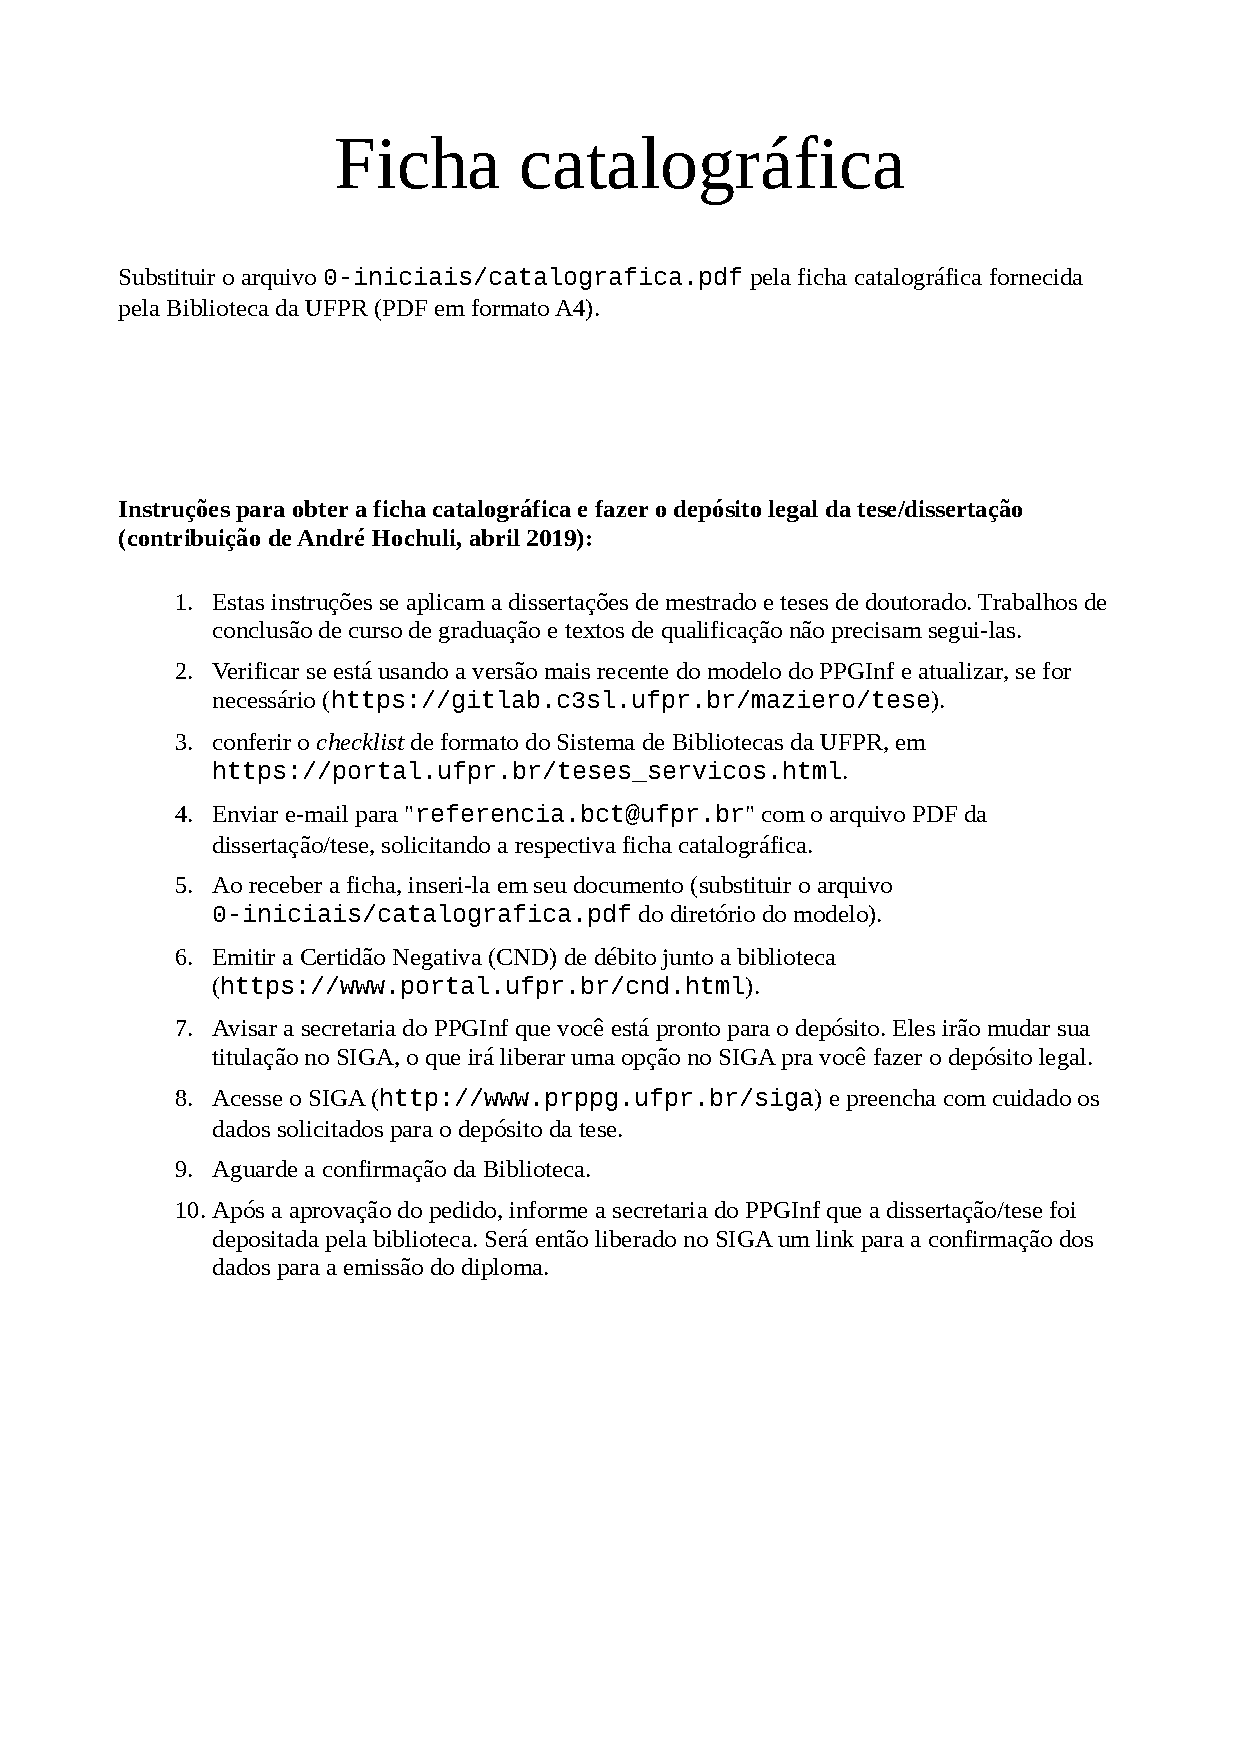
\includepdf[noautoscale]{0-iniciais/catalografica.pdf}

\end{ficha}

%=====================================================
	% ficha catalográfica
% A ficha de aprovação será fornecida pela secretaria do programa,
% após a defesa e cumprimento dos demais trâmites legais.

\begin{aprovacao}	% só gera conteúdo se for na versão final

% inclusão do termo de aprovação final (arquivo PDF)
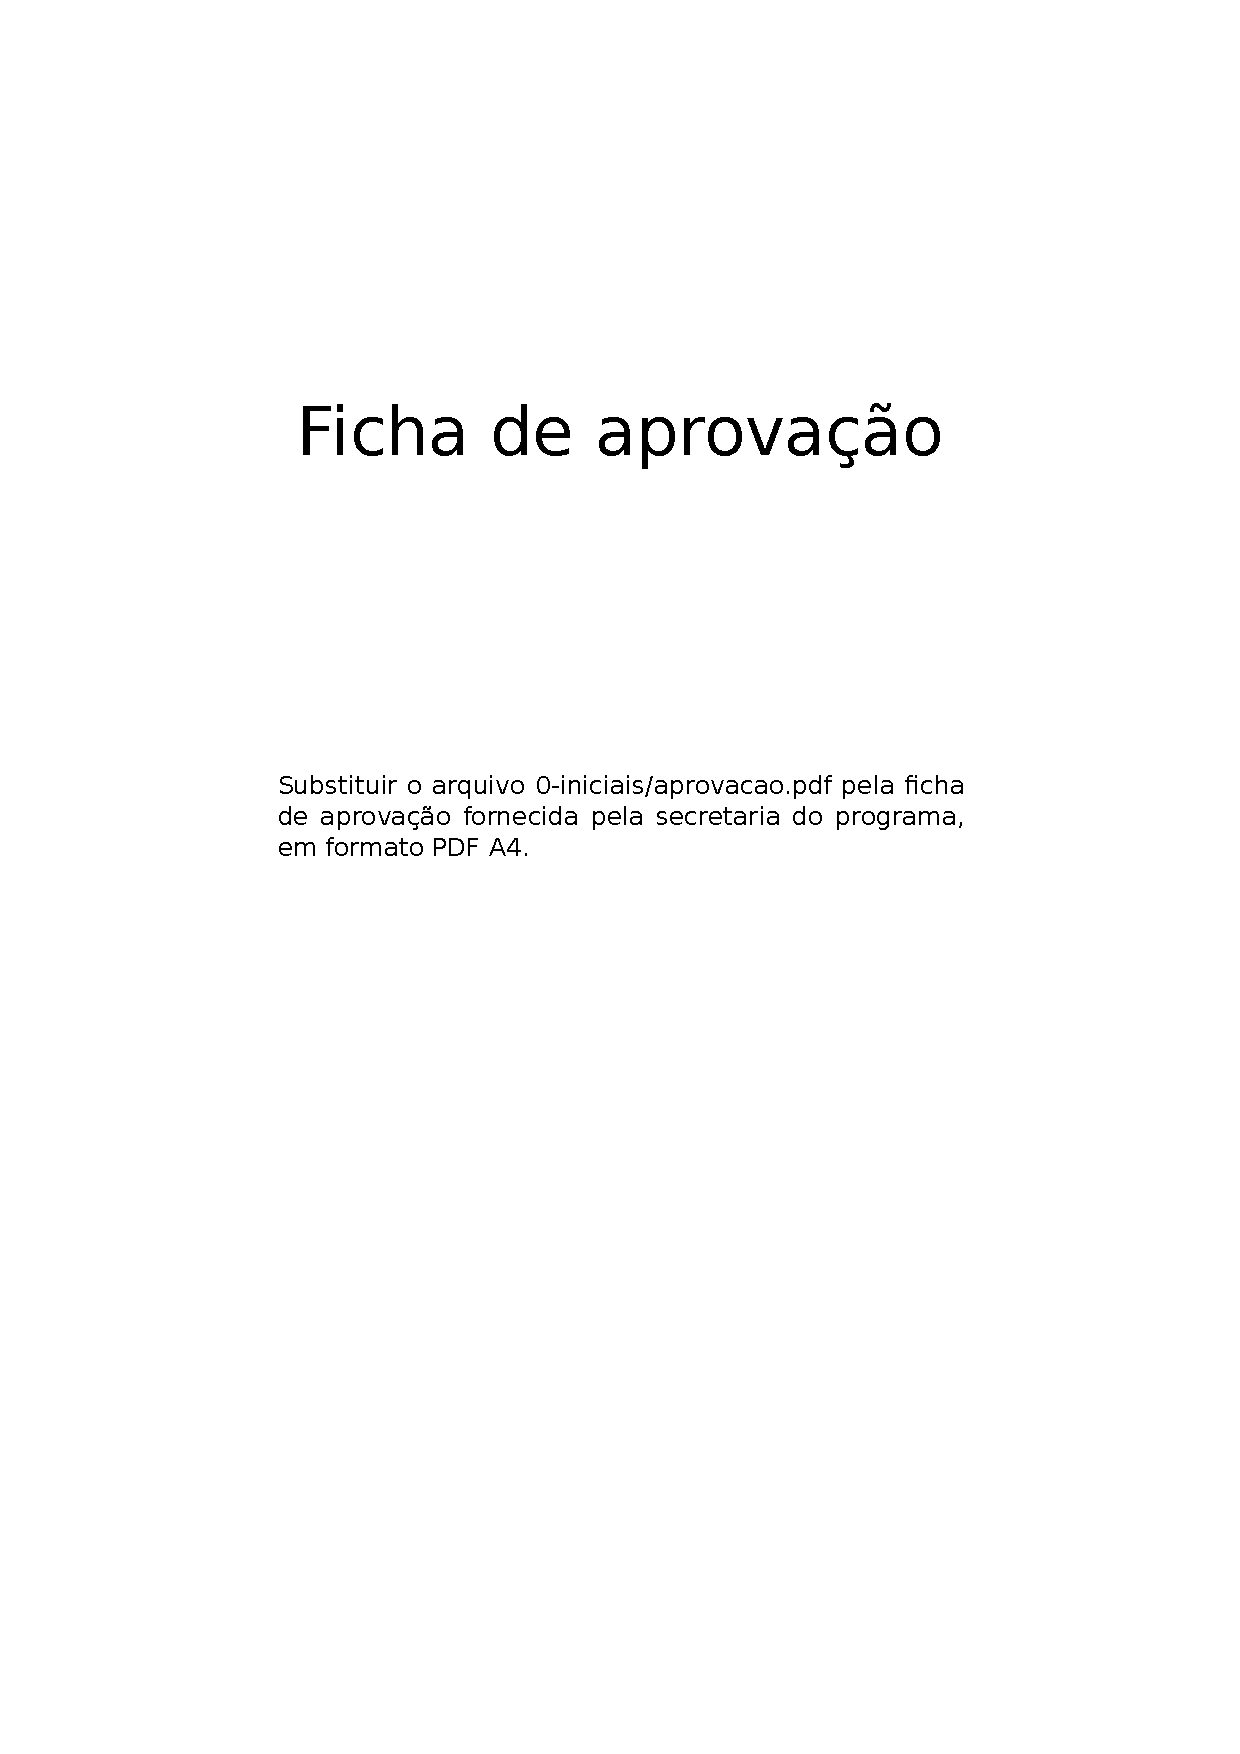
\includepdf[noautoscale]{0-iniciais/aprovacao.pdf}

\end{aprovacao}

%=====================================================
		% folha de aprovação
\begin{dedica}  % só gera conteúdo se for na versão final

A alguém...

\end{dedica}

		% dedicatória
\begin{agradece}	% só gera conteúdo se for na versão final

%Inserir os agradecimentos. Os agradecimentos devem ocupar no máximo uma página, devem ser justificados na largura da página e com um afastamento de parágrafo na primeira linha de 1,27 cm. O espaçamento entre linhas deve ser de 1,5 linhas. Não deve haver espaçamento adicional entre parágrafos.

Equipe Yapira de Robótica UFPR, pela inspiração.


\end{agradece}

		% agradecimentos

% resumo (português) e abstract (inglês)
%\begin{resumo}

O resumo deve conter no máximo 500 palavras, devendo ser justificado na largura da página e escrito em um único parágrafo\footnote{E também não deve ter notas de rodapé; em outras palavras, não siga este exemplo... ;-)} com um afastamento de 1,27 cm na primeira linha. O espaçamento entre linhas deve ser de 1,5 linhas. O resumo deve ser informativo, ou seja, é a condensação do conteúdo e expõe finalidades, metodologia, resultados e conclusões.

%\lipsum[10-13]	% texto aleatório

\end{resumo}

\begin{abstract}

In this paper, we will apply a computer-vision based 3D gaze estimation model on a dataset of driving footage in order to monitor drivers' behaviour.


** STILL IN DEVELOPMENT! **

\end{abstract}


% listas  de figuras, tabelas, abreviações/siglas, símbolos
%\listoffigures				% figuras
%\clearpage
%\listoftables				% tabelas
%%=====================================================

% lista de acrônimos (siglas e abreviações)

\begin{listaacron}

\begin{longtable}[l]{p{0.2\linewidth}p{0.7\linewidth}}
DINF & Departamento de Informática\\
PPGINF & Programa de Pós-Graduação em Informática\\
UFPR & Universidade Federal do Paraná\\
AI & Artificial Intelligence \\
CNN & Convolutional Neural Network

\end{longtable}

\end{listaacron}

%=====================================================
		% acrônimos, deve ser preenchida à mão
%%=====================================================

% lista de símbolos

\begin{listasimb}

\begin{longtable}[l]{p{0.2\linewidth}p{0.7\linewidth}}
$\alpha$ & alfa, primeira letra do alfabeto grego\\
$\beta$ & beta, segunda letra do alfabeto grego\\
$\gamma$ & gama, terceira letra do alfabeto grego\\
$\omega$ & ômega, última letra do alfabeto grego\\
$\pi$ & pi \\
$\tau$ & Tempo de resposta do sistema\\
$\theta$ & Ângulo de incidência do raio luminoso\\
\end{longtable}

\end{listasimb}

%=====================================================
		% símbolos, idem
\tableofcontents			% sumário

%=====================================================

% define estilo do corpo do documento (capítulos e apêndices)
\mainmatter
\pagestyle{mainmatter}

% inclusao de cada capítulo, alterar a gosto (do professor de Metodologia)
\chapter{Introduction}

With upcoming research, gaze estimation is becoming more affordable each passing day, as image-based eye tracking techniques are more accessible than infrared devices. We reached a point in computer vision-based eye tracking research where artificial intelligence models -- such as Gaze360 -- can analyze image data such as head pose and eyeball orientation in order to estimate where humans are looking -- even in unconstrained environments \cite{gaze360_2019}. 

Eye-tracking data can be quite useful for machines. It can be used to train AI models for object-reference or decision-making tasks; used to learn to recognize the context of an image, or even to better understand social cues when interacting with humans \cite{ijcai2020-689}. Current models can also understand abstract concepts such as analysing art paintings by looking where art specialists set their eyes \cite{Massaro2012-jx}.

Intelligent tutoring systems can also automatically detect when students are mind-wandering too, by using gaze features and contextual features such as the teaching subject, the student's score and time spent on each lesson \cite{Hutt2016TheEH}. A similar concept was also applied when monitoring drivers' attention, in an "All in one Network", by using information like head pose, gaze direction, yawning and eye state analysis such as blink rate, blink duration and eye open/close \cite{9053659}.

% ---
% The goal of this paper is to use a novel 3D gaze estimation model, Gaze360 \cite{gaze360_2019}, to extract data on drivers' attention and behaviour on the FDUDrivers Dataset, a dataset containing footage of more than 100 different drivers \cite{9053659}.

% The goal of this paper is to use a novel 3D gaze estimation model, Gaze360 \cite{gaze360_2019}, to extract data on drivers' attention and behaviour on the SynDD1, a dataset containing footage of 10 different drivers from 3 different camera angles, performing various activities \cite{https://doi.org/10.48550/arxiv.2204.08096}.

The goal of this paper is to use a novel 3D gaze estimation model, L2CS-Net \cite{https://doi.org/10.48550/arxiv.2203.03339}, to extract data on drivers' attention and behaviour on driving footage from the DMD - Driver Monitoring Dataset, a dataset made from more than 35 different drivers, from 3 different camera angles with more than 40 hours of real-life driving \cite{jOrtega2020}.			% introdução
\chapter{Alguns exemplos}
\label{cap:exemplos}

% figuras estão no subdiretório "figuras/" dentro deste capítulo
\graphicspath{\currfiledir/figuras/}

%=====================================================

\section{Guias de \LaTeX}

Este modelo contém exemplos para os padrões de inserção de figuras, tabelas, listas de itens, bibliografia, etc. Em caso de dúvidas ou discordância, Pode-se entrar em contato com a direção ou secretaria do programa. Obviamente, críticas (construtivas) e sugestões são muito bem-vindas.

Para aprender a usar \LaTeX, um bom guia introdutório disponível na Internet é \cite{oetiker07}, que também tem uma versão em português. Para tópicos mais avançados consulte \cite{goossens93}.

%=====================================================

\section{Estrutura do texto}

Para melhorar a legibilidade do texto, deve ser evitado o uso de subdivisões mais profundas que a subseção (por exemplo, subsubseções). Se elas forem absolutamente necessarias, não devem ser numeradas. Deve-se analisar a possibilidade de uso de uma lista de itens em seu lugar. O número de níveis de texto do documento não deve exceder três: capítulo, seção e subseção. O uso de mais que três níveis dificulta a leitura e prejudica muito a estética do texto.

%=====================================================

\section{Estilo de redação}

Ao elaborar o texto da dissertação ou da tese, o mais indicado é o uso do verbo na forma impessoal. Exemplos:

\begin{itemize}
\item ... utilizaram-se os seguintes dados ...
\item ... elaborou-se de forma precisa ...
\item ... trata-se os algoritmos ...
\item ... foram obtidos resultados significativos ...
\end{itemize}

Além disso, deve-se a todo custo evitar a ``linguagem de revista'', com expressões como ``sensacional'', ``impressionante'', ``monstruoso'', etc (por exemplo: ``Os resultados obtidos são sensacionais, sobretudo considerando a monstruosa margem de erro.'').

%=====================================================

\section{Alguns exemplos}

Esta seção traz algus exemplos de elementos típicos de um texto científico, como figuras, tabelas e fórmulas matemáticas.

%=====================================================

\subsection{Exemplo de figura}

A forma sugerida para incluir figuras em um documento \LaTeX\ é importá-las usando o pacote \texttt{graphicx}. Como formatos gráficos sugere-se:

\begin{itemize}

\item Formatos \emph{raster}, como PNG (\emph{Portable Network Graphics}) ou JPG (\emph{Joint Photographic Experts Group}) para fotografias; procure usar uma resolução de ao menos 150 dpi (\emph{dots per inch}).

\item Formatos vetoriais, como PDF (\emph{Portable Document Format}) ou EPS (\emph{Extended PostScript}) para diagramas e gráficos\footnote{NUNCA use JPG ou GIF para desenhos vetoriais, pois o resultado final geralmente fica borrado.}.

\end{itemize}

A maior parte das ferramentas permite exportar figuras nesses formatos (a figura do exemplo foi produzida com o \emph{Inkscape}, um programa livre multiplataforma). A figura \ref{fig:comun-intra-inter} mostra um exemplo de inclusão de figura em PDF.

% exemplo de inserção de figura
\begin{figure}[!htb]
\centering
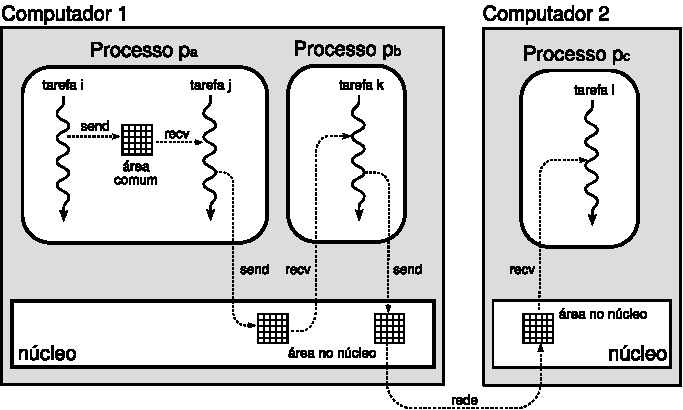
\includegraphics[width=12cm]{exemplo-figura.pdf}
\caption{Comunicação inter-processos.}
\label{fig:comun-intra-inter}
\end{figure}

Para mais informações consulte \cite{goossens93}.

%=====================================================

\subsection{Exemplo de tabela}

Tabelas são elementos importantes de um documento. No \LaTeX\ as tabelas podem ser objetos flutuantes (definidas no ambiente \texttt{table} e referenciadas por números usando \texttt{label} e \texttt{ref}) ou objetos fixos simples, criados pelo ambiente \texttt{tabular}. A tabela \ref{tab:modelos} é um exemplo de tabela flutuante, cuja posição no texto pode variar em função das quebras de página.

\begin{table}[!htp]
\centering
\caption{Os 16 modelos centrais do UCON$_{\mathrm{ABC}}$}
\label{tab:modelos}
\begin{tabular}{|c|cccc|}
\cline{2-5}
\multicolumn{1}{c|}{}& 0 (imutável) & 1 (\emph{pre-update}) & 2 (\emph{on-update}) & 3 (\emph{pos-update}) \\
\hline
\texttt{preA} & \textbullet & \textbullet & -- & \textbullet \\
\hline
\texttt{onA} & \textbullet & \textbullet & \textbullet & \textbullet \\
\hline
\texttt{preB} & \textbullet & \textbullet & -- & \textbullet \\
\hline
\texttt{onB} & \textbullet & \textbullet & \textbullet & \textbullet \\
\hline
\texttt{preC} & \textbullet & -- & -- & -- \\
\hline
\texttt{onC} & \textbullet & -- & -- & -- \\
\hline
\end{tabular}
\end{table}

%=====================================================

\subsection{Exemplo de fórmula}

Equações destacadas devem ser numeradas como mostra a equação \ref{eq:relatividade}:

\begin{equation}
E = m \times c^2
\label{eq:relatividade}
\end{equation}

%=====================================================

\subsection{Exemplos de código-fonte}

Códigos-fonte podem ser produzidos de forma simples através do ambiente \texttt{verbatim}, como mostra este exemplo:

\begin{footnotesize}
\begin{verbatim}
#include <stdio.h>

int main (int argc, char *argv[])
{
   int i ;                           // uma variavel local

   for (i=0; i< 100; i++)            // um laço for
      printf ("i vale %d\n", i) ;    // uma saída na tela
}
\end{verbatim}
\end{footnotesize}

No entanto, é preferível usar pacotes especializados para a edição ou inclusão de códigos-fonte, como o pacote \texttt{listings}. Eis um exemplo de código-fonte escrito com esse pacote:

% exemplo de código-fonte definido no próprio texto

\begin{lstlisting}
#include <stdio.h>

int main (int argc, char *argv[])
{
   int i ;                           // uma variável local

   for (i=0; i< 100; i++)            // um laço for
      printf ("i vale %d\n", i) ;    // uma saída na tela
}
\end{lstlisting}

Esse pacote também permite incluir códigos-fonte de arquivos externos. Eis um exemplo:

% exemplo de código-fonte incluso

\lstinputlisting{2-fundam/exemplo.c}

%=====================================================

\subsection{Exemplo de algoritmo}

Os pacotes \texttt{algorithm} e \texttt{algorithmic} permitem formatar algoritmos facilmente. Eis um exemplo:

\begin{algorithm}[H]
\caption{Ações de $s_i$ ao encerrar um ciclo:}
\label{alg:on-period-ending}
\begin{small}
\begin{algorithmic}[1]
\FORALL{$x \in \mathcal{K}_i$}
  \STATE{$\mathit{banned}_i(x) \gets$ FALSE}
  \STATE{$mi_i(x) \gets 0$}
  \STATE{$mm_i(x) \gets 0$}
  \STATE{$\mathit{age}_i(x) \gets \mathit{age}_i(x) + 1$}
  \IF{$\mathit{age}_i(x) = \mathit{age}_\mathit{max}$}
     \STATE{$\mathcal{K}_i \gets \mathcal{K}_i - \{x\}$}
     \COMMENT{``esquece'' do servidor $x$}
     \STATE{remove as informações locais sobre $x$}
     \STATE{envia $\mathit{notify}(x,\mathit{undef})$ ao grupo de confiança $\mathcal{T}_i$}
  \ENDIF
\ENDFOR
\end{algorithmic}
\end{small}
\end{algorithm}
 
%=====================================================

\subsection{Exemplo de citação}

Como afirmou Maquiavel em seu livro \emph{O Príncipe}:

\begin{quote}
``Nada é mais difícil de instituir, mais perigoso de conduzir, mais incerto no seu sucesso, do que liderar a introdução de uma nova ordem de coisas... O inovador faz inimigos em todos aqueles que prosperavam sobre as antigas regras, e somente tíbio suporte é esperado daqueles que prosperariam na novidade, porque os homens são geralmente incrédulos, nunca realmente confiam nas coisas novas, a menos que as tenham testado em experiência''.
\end{quote}

%=====================================================

\section{Uma seção}

\subsection{Uma subseção}

\subsubsection{Uma subsubseção}

%=====================================================

\section{Conclusão}

Todo capítulo (com exceção da introdução e da conclusão) deve encerrar com uma pequena conclusão local, resumindo os tópicos apresentados no capítulo e preparando o leitor para o próximo capítulo (exceto se esse for a conclusão geral). Caso o capítulo tenha apresentado resultados obtidos pelo próprio autor, estes devem ser sucintamente relembrados aqui.

%=====================================================
		% fundamentação teórica
%\chapter{Testes de alinhamento de listas}

%=====================================================

\section{Outra seção}

Exemplo de lista simples com dois níveis: Exemplo de lista simples com dois níveis: Exemplo de lista simples com dois níveis: Exemplo de lista simples com dois níveis: Exemplo de lista simples com dois níveis: Exemplo de lista simples com dois níveis: Exemplo de lista simples com dois níveis: Exemplo de lista simples com dois níveis: Exemplo de lista simples com dois níveis.

\begin{itemize}

\item Banana, Banana, Banana, Banana, Banana, Banana, Banana, Banana, Banana, Banana, Banana, Banana, Banana, Banana, Banana, Banana, Banana, Banana, Banana, Banana, Banana, Banana, Banana, Banana.

\begin{itemize}

\item Caturra, Caturra, Caturra, Caturra, Caturra, Caturra, Caturra, Caturra, Caturra, Caturra, Caturra, Caturra, Caturra, Caturra, Caturra, Caturra, Caturra, Caturra, Caturra.

\item da Terra, da Terra, da Terra, da Terra, da Terra, da Terra, da Terra, da Terra, da Terra, da Terra, da Terra, da Terra, da Terra, da Terra, da Terra, da Terra, da Terra, da Terra.

\end{itemize}

\item Laranja, Laranja, Laranja, Laranja, Laranja, Laranja, Laranja, Laranja, Laranja, Laranja, Laranja, Laranja, Laranja, Laranja, Laranja, Laranja.

\begin{itemize}

\item Bahia, Bahia, Bahia, Bahia, Bahia, Bahia, Bahia, Bahia, Bahia, Bahia, Bahia, Bahia, Bahia, Bahia, Bahia, Bahia, Bahia, Bahia.

\item Lima, Lima, Lima, Lima, Lima, Lima, Lima, Lima, Lima, Lima, Lima, Lima, Lima, Lima, Lima, Lima, Lima, Lima, Lima, Lima, Lima, Lima, Lima, Lima, Lima, Lima, Lima, Lima, Lima.

\end{itemize}

\end{itemize}

Exemplo de lista numerada com dois níveis: Exemplo de lista numerada com dois níveis: Exemplo de lista numerada com dois níveis: Exemplo de lista numerada com dois níveis: Exemplo de lista numerada com dois níveis: Exemplo de lista numerada com dois níveis: Exemplo de lista numerada com dois níveis: Exemplo de lista numerada com dois níveis.

\begin{enumerate}

\item Banana, Banana, Banana, Banana, Banana, Banana, Banana, Banana, Banana, Banana, Banana, Banana, Banana, Banana, Banana, Banana, Banana, Banana, Banana, Banana, Banana, Banana, Banana, Banana.

\begin{enumerate}

\item Caturra, Caturra, Caturra, Caturra, Caturra, Caturra, Caturra, Caturra, Caturra, Caturra, Caturra, Caturra, Caturra, Caturra, Caturra, Caturra, Caturra, Caturra, Caturra.

\item da Terra, da Terra, da Terra, da Terra, da Terra, da Terra, da Terra, da Terra, da Terra, da Terra, da Terra, da Terra, da Terra, da Terra, da Terra, da Terra, da Terra, da Terra.

\end{enumerate}

\item Laranja, Laranja, Laranja, Laranja, Laranja, Laranja, Laranja, Laranja, Laranja, Laranja, Laranja, Laranja, Laranja, Laranja, Laranja, Laranja.

\begin{enumerate}

\item Bahia, Bahia, Bahia, Bahia, Bahia, Bahia, Bahia, Bahia, Bahia, Bahia, Bahia, Bahia, Bahia, Bahia, Bahia, Bahia, Bahia, Bahia.

\item Lima, Lima, Lima, Lima, Lima, Lima, Lima, Lima, Lima, Lima, Lima, Lima, Lima, Lima, Lima, Lima, Lima, Lima, Lima, Lima, Lima, Lima, Lima, Lima, Lima, Lima, Lima, Lima, Lima.

\end{enumerate}

\end{enumerate}

Exemplo de lista descritiva com dois níveis: Exemplo de lista descritiva com dois níveis: Exemplo de lista descritiva com dois níveis: Exemplo de lista descritiva com dois níveis: Exemplo de lista descritiva com dois níveis: Exemplo de lista descritiva com dois níveis: Exemplo de lista descritiva com dois níveis: Exemplo de lista descritiva com dois níveis: Exemplo de lista descritiva com dois níveis.

\begin{description}

\item [Banana]: Banana, Banana, Banana, Banana, Banana, Banana, Banana, Banana, Banana, Banana, Banana, Banana, Banana, Banana, Banana, Banana, Banana, Banana, Banana, Banana, Banana, Banana, Banana.

\begin{description}

\item [Caturra]: Caturra, Caturra, Caturra, Caturra, Caturra, Caturra, Caturra, Caturra, Caturra, Caturra, Caturra, Caturra, Caturra, Caturra, Caturra, Caturra, Caturra, Caturra.

\item [da Terra]: da Terra, da Terra, da Terra, da Terra, da Terra, da Terra, da Terra, da Terra, da Terra, da Terra, da Terra, da Terra, da Terra, da Terra, da Terra, da Terra, da Terra.

\end{description}

\item [Laranja]: Laranja, Laranja, Laranja, Laranja, Laranja, Laranja, Laranja, Laranja, Laranja, Laranja, Laranja, Laranja, Laranja, Laranja, Laranja.

\begin{description}

\item [Bahia]: Bahia, Bahia, Bahia, Bahia, Bahia, Bahia, Bahia, Bahia, Bahia, Bahia, Bahia, Bahia, Bahia, Bahia, Bahia, Bahia, Bahia.

\item [Lima]: Lima, Lima, Lima, Lima, Lima, Lima, Lima, Lima, Lima, Lima, Lima, Lima, Lima, Lima, Lima, Lima, Lima, Lima, Lima, Lima, Lima, Lima, Lima, Lima, Lima, Lima, Lima, Lima.

\end{description}

\end{description}

%=====================================================
			% estado da arte
%\chapter{Testes de alinhamento de listas}

%=====================================================

\section{Outra seção}

Exemplo de lista simples com dois níveis: Exemplo de lista simples com dois níveis: Exemplo de lista simples com dois níveis: Exemplo de lista simples com dois níveis: Exemplo de lista simples com dois níveis: Exemplo de lista simples com dois níveis: Exemplo de lista simples com dois níveis: Exemplo de lista simples com dois níveis: Exemplo de lista simples com dois níveis.

\begin{itemize}

\item Banana, Banana, Banana, Banana, Banana, Banana, Banana, Banana, Banana, Banana, Banana, Banana, Banana, Banana, Banana, Banana, Banana, Banana, Banana, Banana, Banana, Banana, Banana, Banana.

\begin{itemize}

\item Caturra, Caturra, Caturra, Caturra, Caturra, Caturra, Caturra, Caturra, Caturra, Caturra, Caturra, Caturra, Caturra, Caturra, Caturra, Caturra, Caturra, Caturra, Caturra.

\item da Terra, da Terra, da Terra, da Terra, da Terra, da Terra, da Terra, da Terra, da Terra, da Terra, da Terra, da Terra, da Terra, da Terra, da Terra, da Terra, da Terra, da Terra.

\end{itemize}

\item Laranja, Laranja, Laranja, Laranja, Laranja, Laranja, Laranja, Laranja, Laranja, Laranja, Laranja, Laranja, Laranja, Laranja, Laranja, Laranja.

\begin{itemize}

\item Bahia, Bahia, Bahia, Bahia, Bahia, Bahia, Bahia, Bahia, Bahia, Bahia, Bahia, Bahia, Bahia, Bahia, Bahia, Bahia, Bahia, Bahia.

\item Lima, Lima, Lima, Lima, Lima, Lima, Lima, Lima, Lima, Lima, Lima, Lima, Lima, Lima, Lima, Lima, Lima, Lima, Lima, Lima, Lima, Lima, Lima, Lima, Lima, Lima, Lima, Lima, Lima.

\end{itemize}

\end{itemize}

Exemplo de lista numerada com dois níveis: Exemplo de lista numerada com dois níveis: Exemplo de lista numerada com dois níveis: Exemplo de lista numerada com dois níveis: Exemplo de lista numerada com dois níveis: Exemplo de lista numerada com dois níveis: Exemplo de lista numerada com dois níveis: Exemplo de lista numerada com dois níveis.

\begin{enumerate}

\item Banana, Banana, Banana, Banana, Banana, Banana, Banana, Banana, Banana, Banana, Banana, Banana, Banana, Banana, Banana, Banana, Banana, Banana, Banana, Banana, Banana, Banana, Banana, Banana.

\begin{enumerate}

\item Caturra, Caturra, Caturra, Caturra, Caturra, Caturra, Caturra, Caturra, Caturra, Caturra, Caturra, Caturra, Caturra, Caturra, Caturra, Caturra, Caturra, Caturra, Caturra.

\item da Terra, da Terra, da Terra, da Terra, da Terra, da Terra, da Terra, da Terra, da Terra, da Terra, da Terra, da Terra, da Terra, da Terra, da Terra, da Terra, da Terra, da Terra.

\end{enumerate}

\item Laranja, Laranja, Laranja, Laranja, Laranja, Laranja, Laranja, Laranja, Laranja, Laranja, Laranja, Laranja, Laranja, Laranja, Laranja, Laranja.

\begin{enumerate}

\item Bahia, Bahia, Bahia, Bahia, Bahia, Bahia, Bahia, Bahia, Bahia, Bahia, Bahia, Bahia, Bahia, Bahia, Bahia, Bahia, Bahia, Bahia.

\item Lima, Lima, Lima, Lima, Lima, Lima, Lima, Lima, Lima, Lima, Lima, Lima, Lima, Lima, Lima, Lima, Lima, Lima, Lima, Lima, Lima, Lima, Lima, Lima, Lima, Lima, Lima, Lima, Lima.

\end{enumerate}

\end{enumerate}

Exemplo de lista descritiva com dois níveis: Exemplo de lista descritiva com dois níveis: Exemplo de lista descritiva com dois níveis: Exemplo de lista descritiva com dois níveis: Exemplo de lista descritiva com dois níveis: Exemplo de lista descritiva com dois níveis: Exemplo de lista descritiva com dois níveis: Exemplo de lista descritiva com dois níveis: Exemplo de lista descritiva com dois níveis.

\begin{description}

\item [Banana]: Banana, Banana, Banana, Banana, Banana, Banana, Banana, Banana, Banana, Banana, Banana, Banana, Banana, Banana, Banana, Banana, Banana, Banana, Banana, Banana, Banana, Banana, Banana.

\begin{description}

\item [Caturra]: Caturra, Caturra, Caturra, Caturra, Caturra, Caturra, Caturra, Caturra, Caturra, Caturra, Caturra, Caturra, Caturra, Caturra, Caturra, Caturra, Caturra, Caturra.

\item [da Terra]: da Terra, da Terra, da Terra, da Terra, da Terra, da Terra, da Terra, da Terra, da Terra, da Terra, da Terra, da Terra, da Terra, da Terra, da Terra, da Terra, da Terra.

\end{description}

\item [Laranja]: Laranja, Laranja, Laranja, Laranja, Laranja, Laranja, Laranja, Laranja, Laranja, Laranja, Laranja, Laranja, Laranja, Laranja, Laranja.

\begin{description}

\item [Bahia]: Bahia, Bahia, Bahia, Bahia, Bahia, Bahia, Bahia, Bahia, Bahia, Bahia, Bahia, Bahia, Bahia, Bahia, Bahia, Bahia, Bahia.

\item [Lima]: Lima, Lima, Lima, Lima, Lima, Lima, Lima, Lima, Lima, Lima, Lima, Lima, Lima, Lima, Lima, Lima, Lima, Lima, Lima, Lima, Lima, Lima, Lima, Lima, Lima, Lima, Lima, Lima.

\end{description}

\end{description}

%=====================================================
		% proposta
%\chapter{Testes de alinhamento de listas}

%=====================================================

\section{Outra seção}

Exemplo de lista simples com dois níveis: Exemplo de lista simples com dois níveis: Exemplo de lista simples com dois níveis: Exemplo de lista simples com dois níveis: Exemplo de lista simples com dois níveis: Exemplo de lista simples com dois níveis: Exemplo de lista simples com dois níveis: Exemplo de lista simples com dois níveis: Exemplo de lista simples com dois níveis.

\begin{itemize}

\item Banana, Banana, Banana, Banana, Banana, Banana, Banana, Banana, Banana, Banana, Banana, Banana, Banana, Banana, Banana, Banana, Banana, Banana, Banana, Banana, Banana, Banana, Banana, Banana.

\begin{itemize}

\item Caturra, Caturra, Caturra, Caturra, Caturra, Caturra, Caturra, Caturra, Caturra, Caturra, Caturra, Caturra, Caturra, Caturra, Caturra, Caturra, Caturra, Caturra, Caturra.

\item da Terra, da Terra, da Terra, da Terra, da Terra, da Terra, da Terra, da Terra, da Terra, da Terra, da Terra, da Terra, da Terra, da Terra, da Terra, da Terra, da Terra, da Terra.

\end{itemize}

\item Laranja, Laranja, Laranja, Laranja, Laranja, Laranja, Laranja, Laranja, Laranja, Laranja, Laranja, Laranja, Laranja, Laranja, Laranja, Laranja.

\begin{itemize}

\item Bahia, Bahia, Bahia, Bahia, Bahia, Bahia, Bahia, Bahia, Bahia, Bahia, Bahia, Bahia, Bahia, Bahia, Bahia, Bahia, Bahia, Bahia.

\item Lima, Lima, Lima, Lima, Lima, Lima, Lima, Lima, Lima, Lima, Lima, Lima, Lima, Lima, Lima, Lima, Lima, Lima, Lima, Lima, Lima, Lima, Lima, Lima, Lima, Lima, Lima, Lima, Lima.

\end{itemize}

\end{itemize}

Exemplo de lista numerada com dois níveis: Exemplo de lista numerada com dois níveis: Exemplo de lista numerada com dois níveis: Exemplo de lista numerada com dois níveis: Exemplo de lista numerada com dois níveis: Exemplo de lista numerada com dois níveis: Exemplo de lista numerada com dois níveis: Exemplo de lista numerada com dois níveis.

\begin{enumerate}

\item Banana, Banana, Banana, Banana, Banana, Banana, Banana, Banana, Banana, Banana, Banana, Banana, Banana, Banana, Banana, Banana, Banana, Banana, Banana, Banana, Banana, Banana, Banana, Banana.

\begin{enumerate}

\item Caturra, Caturra, Caturra, Caturra, Caturra, Caturra, Caturra, Caturra, Caturra, Caturra, Caturra, Caturra, Caturra, Caturra, Caturra, Caturra, Caturra, Caturra, Caturra.

\item da Terra, da Terra, da Terra, da Terra, da Terra, da Terra, da Terra, da Terra, da Terra, da Terra, da Terra, da Terra, da Terra, da Terra, da Terra, da Terra, da Terra, da Terra.

\end{enumerate}

\item Laranja, Laranja, Laranja, Laranja, Laranja, Laranja, Laranja, Laranja, Laranja, Laranja, Laranja, Laranja, Laranja, Laranja, Laranja, Laranja.

\begin{enumerate}

\item Bahia, Bahia, Bahia, Bahia, Bahia, Bahia, Bahia, Bahia, Bahia, Bahia, Bahia, Bahia, Bahia, Bahia, Bahia, Bahia, Bahia, Bahia.

\item Lima, Lima, Lima, Lima, Lima, Lima, Lima, Lima, Lima, Lima, Lima, Lima, Lima, Lima, Lima, Lima, Lima, Lima, Lima, Lima, Lima, Lima, Lima, Lima, Lima, Lima, Lima, Lima, Lima.

\end{enumerate}

\end{enumerate}

Exemplo de lista descritiva com dois níveis: Exemplo de lista descritiva com dois níveis: Exemplo de lista descritiva com dois níveis: Exemplo de lista descritiva com dois níveis: Exemplo de lista descritiva com dois níveis: Exemplo de lista descritiva com dois níveis: Exemplo de lista descritiva com dois níveis: Exemplo de lista descritiva com dois níveis: Exemplo de lista descritiva com dois níveis.

\begin{description}

\item [Banana]: Banana, Banana, Banana, Banana, Banana, Banana, Banana, Banana, Banana, Banana, Banana, Banana, Banana, Banana, Banana, Banana, Banana, Banana, Banana, Banana, Banana, Banana, Banana.

\begin{description}

\item [Caturra]: Caturra, Caturra, Caturra, Caturra, Caturra, Caturra, Caturra, Caturra, Caturra, Caturra, Caturra, Caturra, Caturra, Caturra, Caturra, Caturra, Caturra, Caturra.

\item [da Terra]: da Terra, da Terra, da Terra, da Terra, da Terra, da Terra, da Terra, da Terra, da Terra, da Terra, da Terra, da Terra, da Terra, da Terra, da Terra, da Terra, da Terra.

\end{description}

\item [Laranja]: Laranja, Laranja, Laranja, Laranja, Laranja, Laranja, Laranja, Laranja, Laranja, Laranja, Laranja, Laranja, Laranja, Laranja, Laranja.

\begin{description}

\item [Bahia]: Bahia, Bahia, Bahia, Bahia, Bahia, Bahia, Bahia, Bahia, Bahia, Bahia, Bahia, Bahia, Bahia, Bahia, Bahia, Bahia, Bahia.

\item [Lima]: Lima, Lima, Lima, Lima, Lima, Lima, Lima, Lima, Lima, Lima, Lima, Lima, Lima, Lima, Lima, Lima, Lima, Lima, Lima, Lima, Lima, Lima, Lima, Lima, Lima, Lima, Lima, Lima.

\end{description}

\end{description}

%=====================================================
		% experimentação e validação
%\chapter{Testes de alinhamento de listas}

%=====================================================

\section{Outra seção}

Exemplo de lista simples com dois níveis: Exemplo de lista simples com dois níveis: Exemplo de lista simples com dois níveis: Exemplo de lista simples com dois níveis: Exemplo de lista simples com dois níveis: Exemplo de lista simples com dois níveis: Exemplo de lista simples com dois níveis: Exemplo de lista simples com dois níveis: Exemplo de lista simples com dois níveis.

\begin{itemize}

\item Banana, Banana, Banana, Banana, Banana, Banana, Banana, Banana, Banana, Banana, Banana, Banana, Banana, Banana, Banana, Banana, Banana, Banana, Banana, Banana, Banana, Banana, Banana, Banana.

\begin{itemize}

\item Caturra, Caturra, Caturra, Caturra, Caturra, Caturra, Caturra, Caturra, Caturra, Caturra, Caturra, Caturra, Caturra, Caturra, Caturra, Caturra, Caturra, Caturra, Caturra.

\item da Terra, da Terra, da Terra, da Terra, da Terra, da Terra, da Terra, da Terra, da Terra, da Terra, da Terra, da Terra, da Terra, da Terra, da Terra, da Terra, da Terra, da Terra.

\end{itemize}

\item Laranja, Laranja, Laranja, Laranja, Laranja, Laranja, Laranja, Laranja, Laranja, Laranja, Laranja, Laranja, Laranja, Laranja, Laranja, Laranja.

\begin{itemize}

\item Bahia, Bahia, Bahia, Bahia, Bahia, Bahia, Bahia, Bahia, Bahia, Bahia, Bahia, Bahia, Bahia, Bahia, Bahia, Bahia, Bahia, Bahia.

\item Lima, Lima, Lima, Lima, Lima, Lima, Lima, Lima, Lima, Lima, Lima, Lima, Lima, Lima, Lima, Lima, Lima, Lima, Lima, Lima, Lima, Lima, Lima, Lima, Lima, Lima, Lima, Lima, Lima.

\end{itemize}

\end{itemize}

Exemplo de lista numerada com dois níveis: Exemplo de lista numerada com dois níveis: Exemplo de lista numerada com dois níveis: Exemplo de lista numerada com dois níveis: Exemplo de lista numerada com dois níveis: Exemplo de lista numerada com dois níveis: Exemplo de lista numerada com dois níveis: Exemplo de lista numerada com dois níveis.

\begin{enumerate}

\item Banana, Banana, Banana, Banana, Banana, Banana, Banana, Banana, Banana, Banana, Banana, Banana, Banana, Banana, Banana, Banana, Banana, Banana, Banana, Banana, Banana, Banana, Banana, Banana.

\begin{enumerate}

\item Caturra, Caturra, Caturra, Caturra, Caturra, Caturra, Caturra, Caturra, Caturra, Caturra, Caturra, Caturra, Caturra, Caturra, Caturra, Caturra, Caturra, Caturra, Caturra.

\item da Terra, da Terra, da Terra, da Terra, da Terra, da Terra, da Terra, da Terra, da Terra, da Terra, da Terra, da Terra, da Terra, da Terra, da Terra, da Terra, da Terra, da Terra.

\end{enumerate}

\item Laranja, Laranja, Laranja, Laranja, Laranja, Laranja, Laranja, Laranja, Laranja, Laranja, Laranja, Laranja, Laranja, Laranja, Laranja, Laranja.

\begin{enumerate}

\item Bahia, Bahia, Bahia, Bahia, Bahia, Bahia, Bahia, Bahia, Bahia, Bahia, Bahia, Bahia, Bahia, Bahia, Bahia, Bahia, Bahia, Bahia.

\item Lima, Lima, Lima, Lima, Lima, Lima, Lima, Lima, Lima, Lima, Lima, Lima, Lima, Lima, Lima, Lima, Lima, Lima, Lima, Lima, Lima, Lima, Lima, Lima, Lima, Lima, Lima, Lima, Lima.

\end{enumerate}

\end{enumerate}

Exemplo de lista descritiva com dois níveis: Exemplo de lista descritiva com dois níveis: Exemplo de lista descritiva com dois níveis: Exemplo de lista descritiva com dois níveis: Exemplo de lista descritiva com dois níveis: Exemplo de lista descritiva com dois níveis: Exemplo de lista descritiva com dois níveis: Exemplo de lista descritiva com dois níveis: Exemplo de lista descritiva com dois níveis.

\begin{description}

\item [Banana]: Banana, Banana, Banana, Banana, Banana, Banana, Banana, Banana, Banana, Banana, Banana, Banana, Banana, Banana, Banana, Banana, Banana, Banana, Banana, Banana, Banana, Banana, Banana.

\begin{description}

\item [Caturra]: Caturra, Caturra, Caturra, Caturra, Caturra, Caturra, Caturra, Caturra, Caturra, Caturra, Caturra, Caturra, Caturra, Caturra, Caturra, Caturra, Caturra, Caturra.

\item [da Terra]: da Terra, da Terra, da Terra, da Terra, da Terra, da Terra, da Terra, da Terra, da Terra, da Terra, da Terra, da Terra, da Terra, da Terra, da Terra, da Terra, da Terra.

\end{description}

\item [Laranja]: Laranja, Laranja, Laranja, Laranja, Laranja, Laranja, Laranja, Laranja, Laranja, Laranja, Laranja, Laranja, Laranja, Laranja, Laranja.

\begin{description}

\item [Bahia]: Bahia, Bahia, Bahia, Bahia, Bahia, Bahia, Bahia, Bahia, Bahia, Bahia, Bahia, Bahia, Bahia, Bahia, Bahia, Bahia, Bahia.

\item [Lima]: Lima, Lima, Lima, Lima, Lima, Lima, Lima, Lima, Lima, Lima, Lima, Lima, Lima, Lima, Lima, Lima, Lima, Lima, Lima, Lima, Lima, Lima, Lima, Lima, Lima, Lima, Lima, Lima.

\end{description}

\end{description}

%=====================================================
		% conclusão

%=====================================================

% o estilo de bibliografia é definido no arquivo packages.tex

% ATENÇÃO: evite usar \cite{}; prefira \citep{} e \citet{}

% base de bibliografia (BibTeX)

\bibliography{referencias}
\nocite{*}
%\bibliography{file1,file2,file3} % se tiver mais de um arquivo BibTeX

%=====================================================

% inclusão de apêndices
% \appendix

% inclusão de apêndice
% \chapter{Exemplo de anexo}

%=====================================================

Os apêndices são uma extensão do texto, destacados deste para evitar descontinuidade na sequência lógica ou alongamento excessivo de determinado assunto ou tópico secundário dentro dos capítulos da dissertação ou da tese. São contribuições que servem para esclarecer, complementar, provar ou confirmar as ideias apresentadas no texto dos capítulos e que são importantes para a compreensão dos mesmos.

Todos os apêndices devem vir após as referências bibliográficas e devem ser enumerados por letras maiúsculas (A, B, C, ...).

%=====================================================

% \section{Uma Seção}

% \lipsum[20-23]

%=====================================================

% \subsection{Uma Subseção}

% \lipsum[30-33]

%=====================================================

% \subsubsection{Uma Subsubseção}

% \lipsum[30-33]

%=====================================================


% inclusão de apêndice
% \chapter{Testes de alinhamento de listas}

%=====================================================

\section{Outra seção}

Exemplo de lista simples com dois níveis: Exemplo de lista simples com dois níveis: Exemplo de lista simples com dois níveis: Exemplo de lista simples com dois níveis: Exemplo de lista simples com dois níveis: Exemplo de lista simples com dois níveis: Exemplo de lista simples com dois níveis: Exemplo de lista simples com dois níveis: Exemplo de lista simples com dois níveis.

\begin{itemize}

\item Banana, Banana, Banana, Banana, Banana, Banana, Banana, Banana, Banana, Banana, Banana, Banana, Banana, Banana, Banana, Banana, Banana, Banana, Banana, Banana, Banana, Banana, Banana, Banana.

\begin{itemize}

\item Caturra, Caturra, Caturra, Caturra, Caturra, Caturra, Caturra, Caturra, Caturra, Caturra, Caturra, Caturra, Caturra, Caturra, Caturra, Caturra, Caturra, Caturra, Caturra.

\item da Terra, da Terra, da Terra, da Terra, da Terra, da Terra, da Terra, da Terra, da Terra, da Terra, da Terra, da Terra, da Terra, da Terra, da Terra, da Terra, da Terra, da Terra.

\end{itemize}

\item Laranja, Laranja, Laranja, Laranja, Laranja, Laranja, Laranja, Laranja, Laranja, Laranja, Laranja, Laranja, Laranja, Laranja, Laranja, Laranja.

\begin{itemize}

\item Bahia, Bahia, Bahia, Bahia, Bahia, Bahia, Bahia, Bahia, Bahia, Bahia, Bahia, Bahia, Bahia, Bahia, Bahia, Bahia, Bahia, Bahia.

\item Lima, Lima, Lima, Lima, Lima, Lima, Lima, Lima, Lima, Lima, Lima, Lima, Lima, Lima, Lima, Lima, Lima, Lima, Lima, Lima, Lima, Lima, Lima, Lima, Lima, Lima, Lima, Lima, Lima.

\end{itemize}

\end{itemize}

Exemplo de lista numerada com dois níveis: Exemplo de lista numerada com dois níveis: Exemplo de lista numerada com dois níveis: Exemplo de lista numerada com dois níveis: Exemplo de lista numerada com dois níveis: Exemplo de lista numerada com dois níveis: Exemplo de lista numerada com dois níveis: Exemplo de lista numerada com dois níveis.

\begin{enumerate}

\item Banana, Banana, Banana, Banana, Banana, Banana, Banana, Banana, Banana, Banana, Banana, Banana, Banana, Banana, Banana, Banana, Banana, Banana, Banana, Banana, Banana, Banana, Banana, Banana.

\begin{enumerate}

\item Caturra, Caturra, Caturra, Caturra, Caturra, Caturra, Caturra, Caturra, Caturra, Caturra, Caturra, Caturra, Caturra, Caturra, Caturra, Caturra, Caturra, Caturra, Caturra.

\item da Terra, da Terra, da Terra, da Terra, da Terra, da Terra, da Terra, da Terra, da Terra, da Terra, da Terra, da Terra, da Terra, da Terra, da Terra, da Terra, da Terra, da Terra.

\end{enumerate}

\item Laranja, Laranja, Laranja, Laranja, Laranja, Laranja, Laranja, Laranja, Laranja, Laranja, Laranja, Laranja, Laranja, Laranja, Laranja, Laranja.

\begin{enumerate}

\item Bahia, Bahia, Bahia, Bahia, Bahia, Bahia, Bahia, Bahia, Bahia, Bahia, Bahia, Bahia, Bahia, Bahia, Bahia, Bahia, Bahia, Bahia.

\item Lima, Lima, Lima, Lima, Lima, Lima, Lima, Lima, Lima, Lima, Lima, Lima, Lima, Lima, Lima, Lima, Lima, Lima, Lima, Lima, Lima, Lima, Lima, Lima, Lima, Lima, Lima, Lima, Lima.

\end{enumerate}

\end{enumerate}

Exemplo de lista descritiva com dois níveis: Exemplo de lista descritiva com dois níveis: Exemplo de lista descritiva com dois níveis: Exemplo de lista descritiva com dois níveis: Exemplo de lista descritiva com dois níveis: Exemplo de lista descritiva com dois níveis: Exemplo de lista descritiva com dois níveis: Exemplo de lista descritiva com dois níveis: Exemplo de lista descritiva com dois níveis.

\begin{description}

\item [Banana]: Banana, Banana, Banana, Banana, Banana, Banana, Banana, Banana, Banana, Banana, Banana, Banana, Banana, Banana, Banana, Banana, Banana, Banana, Banana, Banana, Banana, Banana, Banana.

\begin{description}

\item [Caturra]: Caturra, Caturra, Caturra, Caturra, Caturra, Caturra, Caturra, Caturra, Caturra, Caturra, Caturra, Caturra, Caturra, Caturra, Caturra, Caturra, Caturra, Caturra.

\item [da Terra]: da Terra, da Terra, da Terra, da Terra, da Terra, da Terra, da Terra, da Terra, da Terra, da Terra, da Terra, da Terra, da Terra, da Terra, da Terra, da Terra, da Terra.

\end{description}

\item [Laranja]: Laranja, Laranja, Laranja, Laranja, Laranja, Laranja, Laranja, Laranja, Laranja, Laranja, Laranja, Laranja, Laranja, Laranja, Laranja.

\begin{description}

\item [Bahia]: Bahia, Bahia, Bahia, Bahia, Bahia, Bahia, Bahia, Bahia, Bahia, Bahia, Bahia, Bahia, Bahia, Bahia, Bahia, Bahia, Bahia.

\item [Lima]: Lima, Lima, Lima, Lima, Lima, Lima, Lima, Lima, Lima, Lima, Lima, Lima, Lima, Lima, Lima, Lima, Lima, Lima, Lima, Lima, Lima, Lima, Lima, Lima, Lima, Lima, Lima, Lima.

\end{description}

\end{description}

%=====================================================


%=====================================================

\end{document}

%=====================================================
